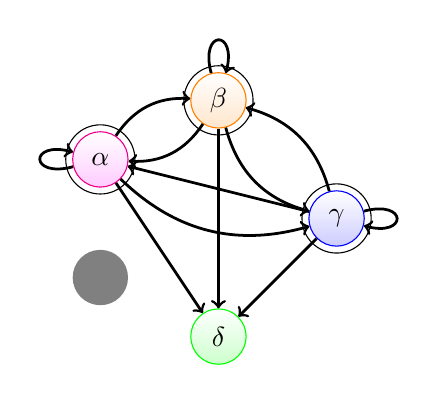
\begin{tikzpicture}[scale=.75]

\tikzset{mynode/.style={circle,minimum size=20pt,inner sep=0pt,draw, top color=white ,bottom color=blue!20, blue,text=black},}
\tikzset{mynode2/.style={circle,minimum size=20pt,inner sep=0pt,draw, top color=white ,bottom color=magenta!20, magenta,text=black},}
\tikzset{mynode3/.style={circle,minimum size=20pt,inner sep=0pt,draw, top color=white ,bottom color=orange!20, orange,text=black},}
\tikzset{mynode6/.style={circle,minimum size=20pt,inner sep=0pt,draw, top color=white ,bottom color=green!20, green,text=black},}
\tikzset{mynode7/.style={circle,fill=gray,minimum size=20pt,inner sep=0pt,},draw}
\tikzset{label/.style={minimum size=15pt,inner sep=0pt,},}

\tikzset{clique/.style={circle,minimum size=25pt,inner sep=0pt,draw}}

%PENTAGONO  
\draw (0,0) node [mynode7] () {};
\draw (0,2) node [mynode2] (alfa1) {$\alpha$};
\draw (4,1) node [mynode] (gamma1) {$\gamma$};
\draw (2,-1) node [mynode6] (delta1) {$\delta$};
\draw (2,3) node [mynode3] (beta1) {$\beta$};

\draw (0,2)node[clique](c1){};
\draw (2,3)node[clique](c1){};
\draw (4,1)node[clique](c1){};     

\draw[->,line width=1pt] (beta1) to[bend left](alfa1);
\draw[->,line width=1pt] (gamma1) -- (alfa1);
\draw[->,line width=1pt] (alfa1) to[bend left](beta1);
\draw[->,line width=1pt] (gamma1)to[bend right](beta1);
\draw[->,line width=1pt] (alfa1) to[bend right] (gamma1);
\draw[->,line width=1pt](beta1)to[bend right]  (gamma1);    
\draw[->,line width=1pt] (alfa1) -- (delta1);
\draw[->,line width=1pt](beta1) -- (delta1);      
\draw[->,line width=1pt](gamma1) -- (delta1);      
\draw[->,line width=1pt] (alfa1) to [loop left] (alfa1);
\draw[->,line width=1pt] (beta1) to [loop above] (beta1);
\draw[->,line width=1pt] (gamma1) to [loop right] (gamma1);

\end{tikzpicture}